\documentclass{article}
\usepackage[paperwidth=841mm,paperheight=1189mm,margin=16mm]{geometry}
\usepackage{type1cm}
\usepackage{amsmath,amssymb}
\usepackage{graphicx}
\usepackage{xcolor}
\usepackage{tikz}
\usetikzlibrary{arrows.meta,positioning}

\pagestyle{empty}
\setlength{\parindent}{0pt}
\setlength{\parskip}{0.16em}
\renewcommand{\familydefault}{\sfdefault}
\graphicspath{{figures/}{logos/}}
\emergencystretch=8em

\definecolor{iasgreen}{RGB}{0,132,61}
\definecolor{iasdark}{RGB}{0,74,38}
\definecolor{topogreen}{RGB}{24,136,74}
\definecolor{topopale}{RGB}{228,244,235}
\definecolor{riskred}{RGB}{184,55,72}
\definecolor{redpale}{RGB}{252,235,238}
\definecolor{warn}{RGB}{194,128,33}
\definecolor{warnpale}{RGB}{255,247,233}
\definecolor{controlblue}{RGB}{42,112,179}
\definecolor{bluepale}{RGB}{232,241,252}
\definecolor{ink}{RGB}{20,31,25}
\definecolor{muted}{RGB}{76,91,84}
\definecolor{linegray}{RGB}{151,166,158}
\definecolor{pale}{RGB}{247,251,248}
\definecolor{paper}{RGB}{255,255,255}
\definecolor{blackband}{RGB}{0,0,0}

\newcommand{\bodyfont}{\fontsize{30}{36}\selectfont}
\newcommand{\smallbody}{\fontsize{25}{31}\selectfont}
\newcommand{\captionfont}{\fontsize{21}{26}\selectfont}
\newcommand{\tinybody}{\fontsize{16}{20}\selectfont}
\newcommand{\blocktitle}[1]{%
  {\fontsize{46}{52}\selectfont\bfseries\color{iasdark}#1}\par
  \vspace{0.12cm}{\color{iasgreen}\rule{\linewidth}{1.5pt}}\par\vspace{0.23cm}
}
\newcommand{\panel}[3]{%
  {\setlength{\fboxsep}{0.42cm}%
  \noindent\fcolorbox{#1}{#2}{%
    \begin{minipage}{\dimexpr\linewidth-2\fboxsep-2\fboxrule\relax}
    \raggedright #3
    \end{minipage}}}%
}
\newcommand{\metric}[4]{%
  {\setlength{\fboxsep}{0.30cm}%
  \fcolorbox{#1}{#2}{%
    \begin{minipage}{\dimexpr\linewidth-2\fboxsep-2\fboxrule\relax}
    \centering
    {\fontsize{38}{44}\selectfont\bfseries\color{#1}#3}\par
    \vspace{0.06cm}
    {\fontsize{22}{28}\selectfont #4}
    \end{minipage}}}%
}
\newcommand{\leverbox}[4]{%
  {\setlength{\fboxsep}{0.30cm}%
  \fcolorbox{#1}{#2}{%
    \begin{minipage}{\dimexpr\linewidth-2\fboxsep-2\fboxrule\relax}
    {\fontsize{29}{35}\selectfont\bfseries\color{#1}#3}\par
    \vspace{0.06cm}
    {\fontsize{23}{29}\selectfont #4}
    \end{minipage}}}%
}

\begin{document}
\bodyfont\color{ink}

% Venue strip
{\setlength{\fboxsep}{0.24cm}
\noindent\colorbox{iasgreen}{%
\begin{minipage}{\dimexpr\textwidth-2\fboxsep\relax}
\color{white}{\fontsize{18}{22}\selectfont\bfseries
IEEE IAS 2026 Annual Meeting \hfill Graduate Student Poster Competition \hfill Vancouver, Canada, Oct 4-8, 2026}
\end{minipage}}}

\vspace{0.35cm}

% Title band
\noindent
\begin{minipage}[c]{0.18\textwidth}
\centering
\includegraphics[width=0.98\linewidth]{ias_annual_2026_logo.png}\\[-0.06cm]
{\tinybody\color{muted}IEEE IAS Annual Meeting 2026}
\end{minipage}\hfill
\begin{minipage}[c]{0.63\textwidth}
\resizebox{\linewidth}{!}{\fontsize{108}{118}\selectfont\bfseries Network or Control?}\par
\vspace{0.12cm}
{\fontsize{51}{59}\selectfont\bfseries A Validated Spectral Bridge for Inverter-Dominated Grids}\par
\vspace{0.14cm}
{\fontsize{31}{37}\selectfont\color{iasdark}Weak-node and weak-link analysis as an application of the controller-aware bridge}\par
\vspace{0.20cm}
{\fontsize{23}{28}\selectfont Jorge L. Mayorga Taborda \quad | \quad Universidad de los Andes, Bogota, Colombia}
\end{minipage}\hfill
\begin{minipage}[c]{0.14\textwidth}
\centering
\includegraphics[width=0.56\linewidth]{repo_qr.png}\\[-0.02cm]
{\fontsize{15}{18}\selectfont\bfseries\color{iasdark}Scan for code and data}\\[-0.02cm]
{\tinybody github.com/jlmayorgaco}
\end{minipage}

\vspace{0.42cm}

% Hook band
{\setlength{\fboxsep}{0.50cm}
\noindent\colorbox{blackband}{%
\begin{minipage}{\dimexpr\textwidth-2\fboxsep\relax}
\centering\color{white}
{\fontsize{66}{76}\selectfont\bfseries
Not every weak node is weak for the same reason. Some need copper; some need control.}
\end{minipage}}}

\vspace{0.36cm}

% Consequence band
\panel{riskred}{redpale}{%
{\fontsize{44}{52}\selectfont\bfseries\color{riskred}Practical consequence for IAS:}\quad
{\fontsize{38}{46}\selectfont
A planner using the standard reduced model can approve an inverter conversion while the true critical control mode stays invisible.}
}

\vspace{0.45cm}

% Main two-column mosaic
\noindent
\begin{minipage}[t]{0.488\textwidth}
\vspace{0pt}

\panel{linegray}{paper}{%
\blocktitle{1. The problem IAS recognizes}
Industrial grids and microgrids are replacing synchronous machines with inverter-based resources. The visible change is lower inertia. The subtle change is damping location.

\vspace{0.18cm}
\begin{minipage}[t]{0.48\linewidth}
\metric{topogreen}{topopale}{Old view}{machine inertia and nodal damping carry the margin}
\end{minipage}\hfill
\begin{minipage}[t]{0.48\linewidth}
\metric{controlblue}{bluepale}{IBR view}{PLL, exciters, governors, stabilizers, inverter loops}
\end{minipage}

\vspace{0.20cm}
\smallbody
Classical weak-node or weak-link screens based on graph participation can identify a stressed place, but they may not identify the reason. The critical mode can belong to the control family, not the network family.
\vspace{1.25cm}
}

\vspace{0.34cm}

\panel{riskred}{redpale}{%
\blocktitle{2. Why the scalar bridge fails}
\smallbody
The standard reduced certificate puts damping into a fixed nodal coefficient \(D\). In the studied ANDES cases,
{\fontsize{36}{43}\selectfont
\[
\texttt{GENROU.D}=0,
\tag{1}
\]
}
yet the full eigensolve has modal damping. The coefficient model lost the damping channel.

\vspace{0.12cm}
\bodyfont
The failure is not numerical. It is a modeling failure: controller states were condensed as if they had no frequency memory.
\vspace{1.45cm}
}

\vspace{0.34cm}

\panel{controlblue}{bluepale}{%
\blocktitle{3. The controller-aware bridge}
\smallbody
Partition the linearized ANDES state matrix into retained network/interface states and condensed control states. The reduced object is the Schur nonlinear eigenproblem
{\fontsize{33}{39}\selectfont
\[
S_e(s)=sI-A_{ee}-A_{ec}(sI-A_{cc})^{-1}A_{ce}.
\tag{2}
\]
}
Equivalently, controller states enter the second-order view as a rational self-energy:
{\fontsize{33}{39}\selectfont
\[
\Sigma(s)=D_0+C(sI-A_{cc})^{-1}B .
\tag{3}
\]
}
The \(s\)-dependence is the point. It keeps controller memory in the reduced spectral problem.
\vspace{1.35cm}
}

\vspace{0.34cm}

\panel{warn}{warnpale}{%
\blocktitle{4. What is classical, what is ours}
\smallbody
Schur complements, Beyn contour extraction, nonlinear eigenvalue problems, and perturbation tools are classical. The contribution here is not new mathematics.

\vspace{0.12cm}
The contribution is the applied formulation and audit: static condensation fails on the relevant cases, rational condensation recovers the critical poles, and the recovered pole family tells the engineer which lever to inspect.
\vspace{1.60cm}
}

\end{minipage}\hfill
\begin{minipage}[t]{0.488\textwidth}
\vspace{0pt}

\panel{iasgreen}{paper}{%
\blocktitle{5. Dominant figure: you were looking in the wrong place}
\centering
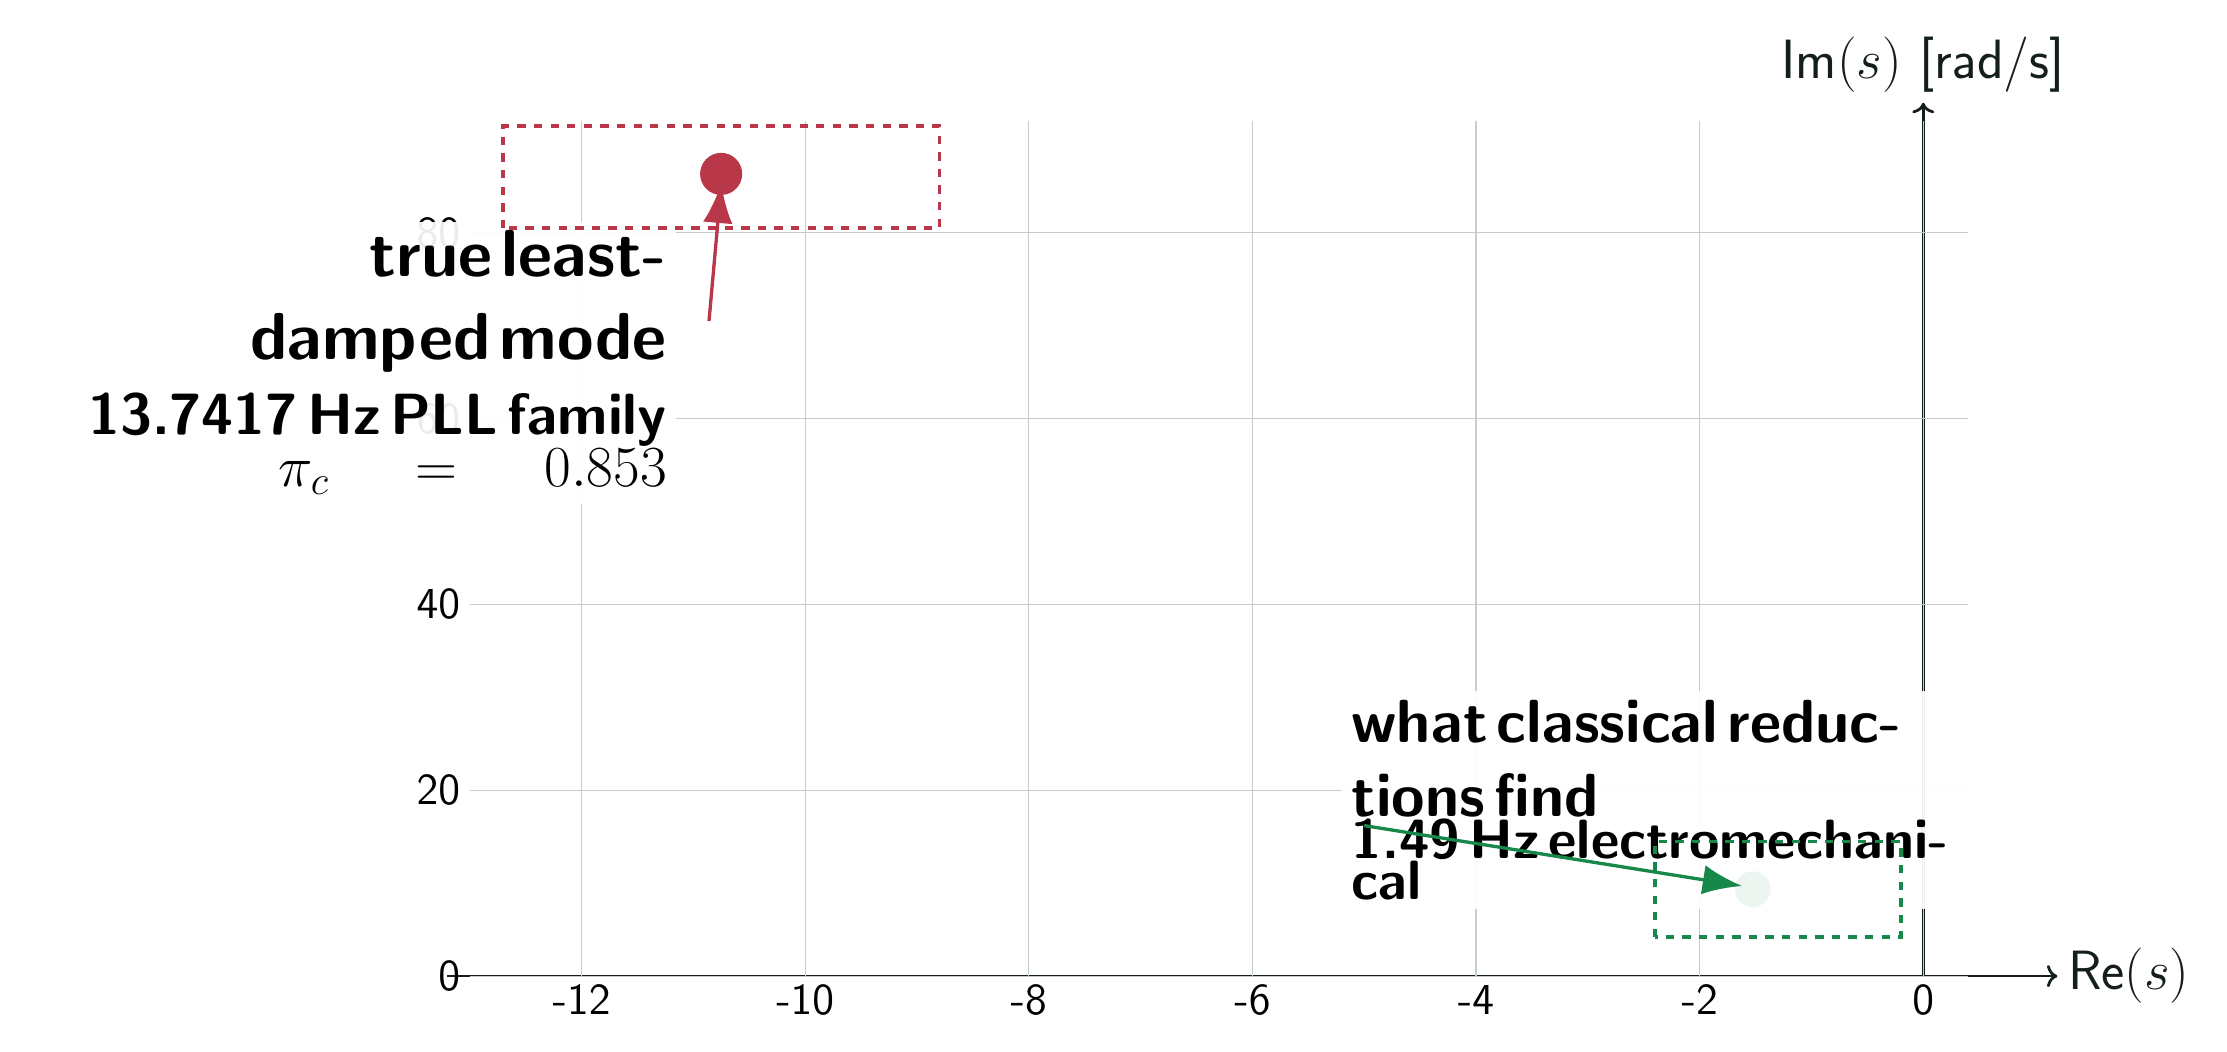
\begin{tikzpicture}[x=1.42cm,y=0.118cm]
  \draw[->,line width=1.0pt,color=ink] (-13.2,0) -- (1.2,0) node[right] {\fontsize{20}{24}\selectfont Re\((s)\)};
  \draw[->,line width=1.0pt,color=ink] (0,0) -- (0,94) node[above] {\fontsize{20}{24}\selectfont Im\((s)\) [rad/s]};
  \foreach \x in {-12,-10,-8,-6,-4,-2,0} {
    \draw[color=linegray!55] (\x,0) -- (\x,92);
    \node[below] at (\x,0) {\fontsize{16}{19}\selectfont \x};
  }
  \foreach \y in {0,20,40,60,80} {
    \draw[color=linegray!55] (-13,\y) -- (0.4,\y);
    \node[left] at (-13,\y) {\fontsize{16}{19}\selectfont \y};
  }
  \filldraw[topogreen] (-1.5256,9.3584) circle (0.22cm);
  \node[anchor=west,align=left,text width=8.2cm,fill=white,fill opacity=0.92,text opacity=1] at (-5.2,19) {\fontsize{22}{27}\selectfont\bfseries what classical reductions find\\\fontsize{20}{25}\selectfont 1.49 Hz electromechanical};
  \draw[-{Latex[length=5mm]},line width=1.2pt,color=topogreen] (-5.0,16.2) -- (-1.62,9.7);

  \filldraw[riskred] (-10.7514,86.3419) circle (0.26cm);
  \node[anchor=east,align=right,text width=8.0cm,fill=white,fill opacity=0.92,text opacity=1] at (-11.15,66) {\fontsize{24}{30}\selectfont\bfseries true least-damped mode\\\fontsize{21}{27}\selectfont 13.7417 Hz PLL family\\\(\pi_c=0.853\)};
  \draw[-{Latex[length=5mm]},line width=1.2pt,color=riskred] (-10.86,70.5) -- (-10.75,85.3);

  \draw[dashed,line width=1.3pt,color=riskred] (-12.7,80.5) rectangle (-8.8,91.5);
  \draw[dashed,line width=1.3pt,color=topogreen] (-2.4,4.2) rectangle (-0.2,14.5);
\end{tikzpicture}

\vspace{0.10cm}
\captionfont
Mix60 audit. A fixed-point/scalar reduction returns the low-frequency electromechanical mode. The full ANDES eigensolve and the rational Schur bridge recover the PLL-family least-damped mode.
\vspace{1.00cm}
}

\vspace{0.34cm}

\panel{iasgreen}{topopale}{%
\blocktitle{6. Validated bridge result}
\smallbody
\begin{minipage}[t]{0.31\linewidth}
\metric{iasgreen}{paper}{no-PSS}{critical pole matched}
\end{minipage}\hfill
\begin{minipage}[t]{0.31\linewidth}
\metric{iasgreen}{paper}{base}{critical pole matched}
\end{minipage}\hfill
\begin{minipage}[t]{0.31\linewidth}
\metric{iasgreen}{paper}{Mix60}{PLL critical pole captured}
\end{minipage}

\vspace{0.20cm}
\begin{minipage}[t]{0.48\linewidth}
\metric{iasgreen}{paper}{\(8.47{\times}10^{-11}\%\)}{worst frequency error}
\end{minipage}\hfill
\begin{minipage}[t]{0.48\linewidth}
\metric{iasgreen}{paper}{\(2.48{\times}10^{-9}\%\)}{worst damping error}
\end{minipage}

\vspace{0.20cm}
\captionfont
Beyn contour extraction of the Schur NEP matches full ANDES critical poles in the three diagnostic cases. This is machine-level numerical agreement for the bridge, not a claim that planning rankings are fully validated.
\vspace{1.10cm}
}

\vspace{0.34cm}

\panel{linegray}{pale}{%
\blocktitle{7. Utility: weak nodes and weak links}
\begin{minipage}[t]{0.32\linewidth}
\leverbox{topogreen}{topopale}{Network weak node}{reinforce topology; copper can move the mode}
\end{minipage}\hfill
\begin{minipage}[t]{0.32\linewidth}
\leverbox{controlblue}{bluepale}{Control weak node}{retune PLL, inverter, governor, or stabilizer}
\end{minipage}\hfill
\begin{minipage}[t]{0.32\linewidth}
\leverbox{riskred}{redpale}{Resonant weak link}{reinforcement can reduce damping}
\end{minipage}

\vspace{0.22cm}
\smallbody
The bridge classifies the weak element by family. That is the decision value: it tells the planner which lever is physically connected to the observed damping margin.

\vspace{0.14cm}
In the line audit, \(40\) strict control-resonant records appeared among \(348\) global-margin-reversal records. Minoritary, but real.
\vspace{1.30cm}
}

\end{minipage}

\vspace{0.50cm}

% Bottom full-width band
\noindent
\begin{minipage}[t]{0.335\textwidth}
\panel{riskred}{redpale}{%
\blocktitle{8. Scope guard}
\smallbody
The bridge is validated to machine-level numerical agreement on diagnostic ANDES cases with generic controls.

\vspace{0.12cm}
The controller-aware weak-element ranking is a formulation. Full ANDES validation over calibrated operating ranges remains in progress.

\vspace{0.12cm}
The resonant weak-link mechanism is modal-local and control-conditional. It is not claimed as a dominant system-wide collapse mechanism.
\vspace{1.70cm}
}
\end{minipage}\hfill
\begin{minipage}[t]{0.305\textwidth}
\panel{controlblue}{bluepale}{%
\blocktitle{9. How the poster sells to IAS}
\smallbody
Problem: damping moved from machines into controls.

\vspace{0.10cm}
Risk: the standard reduced model can certify the wrong mode.

\vspace{0.10cm}
Result: the rational Schur bridge recovers the critical ANDES poles.

\vspace{0.10cm}
Action: decide whether the weakness is network, control, or resonant.
\vspace{2.45cm}
}
\end{minipage}\hfill
\begin{minipage}[t]{0.315\textwidth}
\panel{blackband}{blackband}{%
\color{white}
{\fontsize{46}{52}\selectfont\bfseries Takeaway}\par
\vspace{0.16cm}
{\fontsize{28}{34}\selectfont
Do not ask only where the grid is weak. Ask whether the weakness belongs to the network family or the control family. The fix is different.}

\vspace{0.55cm}
\begin{minipage}[c]{0.30\linewidth}
\includegraphics[width=0.92\linewidth]{repo_qr.png}
\end{minipage}\hfill
\begin{minipage}[c]{0.66\linewidth}
{\fontsize{25}{31}\selectfont\bfseries Reproducibility}\par
{\fontsize{18}{23}\selectfont ANDES gates, NEP contour solver, and line-audit artifacts are included.}\\[-0.02cm]
{\fontsize{15}{19}\selectfont github.com/jlmayorgaco/paper-P06-spectral-graph-power-dynamics}
\end{minipage}
\vspace{1.40cm}
}
\end{minipage}

\vspace{0.45cm}

{\setlength{\fboxsep}{0.42cm}
\noindent\colorbox{iasdark}{%
\begin{minipage}{\dimexpr\textwidth-2\fboxsep\relax}
\centering\color{white}
{\fontsize{40}{48}\selectfont\bfseries Operating rule: classify the pole family first, choose the lever second.}
\quad
{\fontsize{30}{38}\selectfont Network family \(\rightarrow\) topology. Control family \(\rightarrow\) tuning. Resonant link \(\rightarrow\) avoid or retune before reinforcing.}
\end{minipage}}}

\end{document}
